\section{Experiments}\label{sec:experiments}
To demonstrate and evaluate our GeoTracking and GeoRouting, 
we integrated these extensions with the IBRDTN implementation, and performed experiments on 
the VMT channel-emulated testbed~\cite{hahn10:using, kim11:reality}.  

\subsection{VMT Testbed Results}\label{sec:vmtresults}
We ran several experiments on the VirtualMeshTest (VMT)
mobile wireless testbed~\cite{hahn10:using, kim11:reality}.
VMT allows us to subject Linux-based real wireless nodes with commodity 
wireless hardware to emulated mobile environments.  The 
wireless testbed is effectively an analog channel emulator based
on an array of programmable attenuators.  Given a desired physical arrangement
of nodes, the system computes the expected path loss between
nodes and programs the attenuators to achieve those path loss
properties.  By updating the attenuations every second, VMT can
emulate a mobile wireless environment for real wireless nodes.

\subsection{Crop Circles Scenario}



\begin{figure}
\vspace{-.2cm}
\begin{center}
%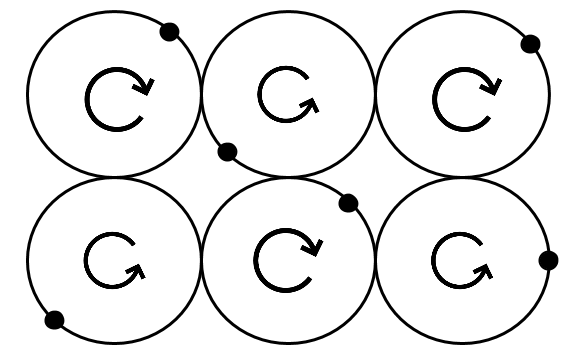
\includegraphics[width=\columnwidth+.5]{figures/cropcircle1.png}
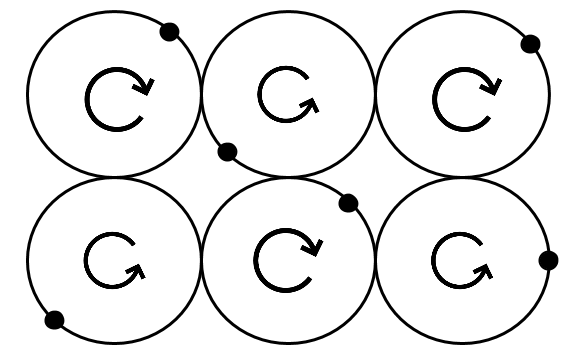
\includegraphics[width=3in]{figures/cropcircle1.png}
\end{center}
\vspace{-.4cm}
\caption{Crop Circles Experiment}\label{fig:cropcircle1}
\vspace{-.35cm}
\end{figure}

The first crop circles mobility scenario consists of six mobile nodes, arranged in two rows. As shown in 
Figure~\ref{fig:cropcircle1}, some nodes follow a circle in a clockwise direction, and some nodes follow a counter-clockwise path. The source in these experiments is the lower left node, and the responder is the upper right node.



%The second crop circles mobility scenario, shown in Figure~\ref{fig:cropcircles2}, consists of eighteen mobile nodes, arranged in six rows. The source in these experiments is Node 1, and the responder is Node 18.
